\newpage
\section{Resultados}
\subsubsection{Regresi\'on Lineal}
\begin{figure}[h!]
	\centering
	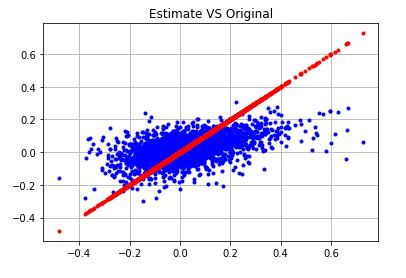
\includegraphics[width=1\linewidth]{Figure/RegresionLineal_Results.JPG}
	\caption{Lag level per group} 
	\label{fig:TrainingDataSet}
\end{figure}
\subsubsection{Decision Tree}

\subsubsection{Random Forest Regressor}
\subsubsection{XGBoost}

\begin{figure}[h!]
	\centering
	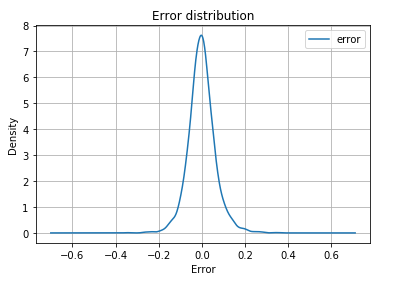
\includegraphics[width=1\linewidth]{Figure/xgbregresor_results.png}
	\caption{Lag level per group} 
	\label{fig:xgbregresor}
\end{figure}

\begin{lstlisting}[language=Python]
xgb_grid.best_params_
{'colsample_bytree': 0.7, 
'learning_rate': 0.07, 
'max_depth': 5, 
'min_child_weight': 4, 
'n_estimators': 100, 
'nthread': 4, 
'objective': 'reg:linear', 
'silent': 1, 
'subsample': 0.7}
\end{lstlisting}
